\documentclass[12pt]{article}
\usepackage[utf8]{inputenc}
\usepackage[T1]{fontenc}
\usepackage{amsmath}
\usepackage{amsfonts}
\usepackage{amssymb}
\usepackage[version=4]{mhchem}
\usepackage{stmaryrd}
\usepackage{graphicx}
\usepackage[export]{adjustbox}
\graphicspath{ {./images/} }

\usepackage{listings} % Required for insertion of code
\usepackage{xcolor} % Required for custom colors

% Define custom colors
\definecolor{codegreen}{rgb}{0,0.6,0}
\definecolor{codegray}{rgb}{0.5,0.5,0.5}
\definecolor{codepurple}{rgb}{0.58,0,0.82}
\definecolor{backcolour}{rgb}{0.95,0.95,0.92}

% Setup the style for code listings
\lstdefinestyle{mystyle}{
    backgroundcolor=\color{backcolour},   
    commentstyle=\color{codegreen},
    keywordstyle=\color{magenta},
    numberstyle=\tiny\color{codegray},
    stringstyle=\color{codepurple},
    basicstyle=\ttfamily\footnotesize,
    breakatwhitespace=false,         
    breaklines=true,                 
    captionpos=b,                    
    keepspaces=true,                 
    numbers=left,                    
    numbersep=5pt,                  
    showspaces=false,                
    showstringspaces=false,
    showtabs=false,                  
    tabsize=2
}

% Activate the style
\lstset{style=mystyle}


\title{Ch14 Winter term 2024 }

\author{}
\date{}


\begin{document}
\maketitle
Problem set 4

due May 23, 2024

for Problems 1 and 2: for $\mathrm{CO}_{2}, \mathrm{HCO}_{3}{ }^{-}, \mathrm{CO}_{3}{ }^{2-}, \mathrm{CaCO}_{3}$ at $25^{\circ} \mathrm{C}$, use

$\mathrm{k}_{\mathrm{H}}=0.035 \mathrm{M} \mathrm{atm}^{-1}, \mathrm{~K}_{\mathrm{a} 1}=4.25 \times 10^{-7}, \mathrm{~K}_{\mathrm{a} 2}=5.01 \times 10^{-11}, \mathrm{~K}_{\mathrm{sp}}=4.5 \times 10^{-9}$

\section{}
Calculate the $\mathrm{pH}$ of the following solutions. The contribution of $\mathrm{H}_{2} \mathrm{CO}_{3}$ to the total concentration of dissolved $\mathrm{CO}_{2}$-related species can be neglected in this analysis; these samples consist only of a solution, with neither gas phase $\mathrm{CO}_{2}$ nor solid $\mathrm{CaCO}_{3}$.

\subsection{}
$20 \mathrm{mM} \mathrm{NaHCO_3}$
\subsubsection{Answer}
This suggests that we have 20 mM of $\mathrm{HCO}_{3}^{-}$. Now we have the equilibrium expression for the dissociation of a proton from $\mathrm{HCO}_{3}^{-}$:
\begin{equation}
\mathrm{HCO}_{3}^{-} \rightleftharpoons \mathrm{H}^{+}+\mathrm{CO}_{3}^{2-}
\end{equation}
The equilibrium constant for this reaction is given by:
\begin{equation}
K_{a}=\frac{[\mathrm{H}^{+}][\mathrm{CO}_{3}^{2-}]}{[\mathrm{HCO}_{3}^{-}]}
\end{equation}
We can consider $0.02 -x $ as the concentration of $\mathrm{HCO}_{3}^{-}$ after dissociation and $x$ as the concentration of $\mathrm{H}^{+}$ and $\mathrm{CO}_{3}^{2-}$. Substituting these values into the equilibrium constant expression, we get:
\begin{equation}
5.01 \times 10^{-11}=\frac{x^{2}}{0.02-x}
\end{equation}
Solving this equation, we get the $\mathrm{pH}$ of the solution is $6.00$.
% Inline Python code in the document
\begin{lstlisting}[language=Python]
import sympy as sp

# Given constants
Ka2 = 5.01e-11
initial_HCO3 = 0.02
x = sp.symbols('x')
final_HCO3 = 0.02 - x
final_H = x
final_CO3 = x
eq = Ka2 - (final_H * final_CO3) / final_HCO3
x = sp.solve(eq, x)
# now get the pH
H = x[0]
pH = -sp.log(H, 10)
pH.evalf()

\end{lstlisting}


\subsection{}
$20 \mathrm{mM} \mathrm{Na}_{2} \mathrm{CO}_{3}$
\subsubsection{Answer}
This suggests that we have 20 mM of $\mathrm{CO}_{3}^{2-}$. We are interested in the hydrolysis of this ionic species in water:
\begin{equation}
\mathrm{CO}_{3}^{2-}+2 \mathrm{H}_{2} \mathrm{O} \rightleftharpoons \mathrm{HCO}_{3}^{-}+\mathrm{OH}^{-}
\end{equation}
We can use the given $K_{a2}$ to determine the $K_{b}$ for the hydrolysis of $\mathrm{CO}_{3}^{2-}$:
\begin{equation}
K_{b}=\frac{K_{w}}{K_{a2}}
\end{equation}
Then the equilibrium expression for this hydrolysis is:
\begin{equation}
K_{b}=\frac{[\mathrm{HCO}_{3}^{-}][\mathrm{OH}^{-}]}{[\mathrm{CO}_{3}^{2-}]}
\end{equation}
This gives a pH of 11.3.
% Inline Python code in the document
\begin{lstlisting}[language=Python]
import sympy as sp

# Given constants
Ka2 = 5.01e-11
# calculate the Kb from the Ka2
Kw = 1e-14
Kb = Kw / Ka2
initial_CO3 = 0.02
x = sp.symbols('x')
final_CO3 = 0.02 - x
final_OH = x
final_HCO3 = x
eq = Kb - (final_OH * final_HCO3) / final_CO3
x = sp.solve(eq, x)
# now get the pOH
OH = x[0]
pOH = -sp.log(OH, 10)
# convert this into a pH
pH = 14 - pOH
pH.evalf()
\end{lstlisting}


\section{}
This problem is modified from the 2022 midterm, problem 6B "Is this a soluble problem?", which, ironically, was not soluble as it was written...

\subsection{}
What partial pressure (in atm) of gas phase $\mathrm{CO}_{2}$ exists in equilibrium with a solution saturated with $\mathrm{CaCO}_{3}$ at $\mathrm{pH}=7.5$ ? The problem originally specified that the free $\mathrm{Ca}^{2+}$ concentration $=0.001$ $\mathrm{M}$, but this constraint is inconsistent with the relevant equilibrium constants.
\subsubsection{Answer}
The solubility product constant for $\mathrm{CaCO}_{3}$ is given by:
\begin{equation}
K_{sp}=[\mathrm{Ca}^{2+}][\mathrm{CO}_{3}^{2-}]
\end{equation}


\section{}
A protein $\mathrm{P}$ binds to DNA according to the following reaction

$$
P^{Z P \pm}+D N A^{Z-} \stackrel{K_{A}}{\rightleftharpoons} P \cdot D N A^{Z-Z P \pm}
$$

where $\mathrm{K}_{\mathrm{A}}$ is the association constant for the binding of $\mathrm{P}$ to DNA. $\mathrm{P}$ has multiple positively charged amino groups and multiple negatively charged carboxylate groups, with an overall charge of $\mathrm{ZP} \pm$. Due to the titration of these ionizable residues, the overall charge $\mathrm{ZP} \pm$ is a function of $\mathrm{pH}$ as shown below:

\begin{center}
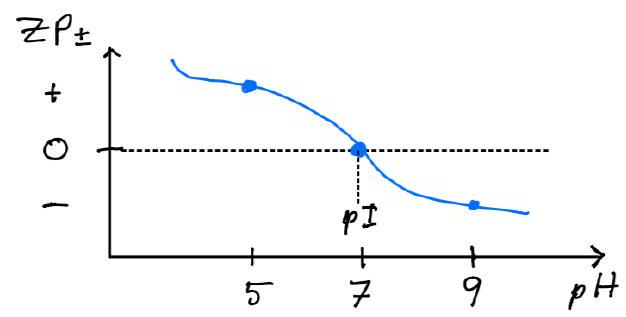
\includegraphics[max width=\textwidth]{2024_05_17_4f752ecd7e7a86925d15g-1}
\end{center}

At the isoelectric point, $\mathrm{pl}$, the positively charged residues are balanced by the negatively charged residues, so that the net charge is 0 . The DNA remains negatively charged at all $\mathrm{pHs}$. The association of $P$ and DNA has a strong electrostatic component based on the net charges of $\mathrm{P}$ and $\mathrm{DNA}$; i.e., at $\mathrm{pHs}$ lower than the $\mathrm{pl}, \mathrm{P}$ has a net positive charge, so there is an attractive electrostatic contribution stabilizing complex formation with the negatively charged DNA, while at $\mathrm{pHs}$ above the $\mathrm{pl}, \mathrm{P}$ has a net negative charge so there is a repulsive electrostatic contribution destabilizing complex formation with DNA. At every $\mathrm{pH}$, the charge of the complex is the sum of the charges on the protein at that $\mathrm{pH}$, plus the negative charge on DNA.

From Ch14, we know that equilibrium concentrations involving charged species will depend on ionic strength (I) due to the ionic strength dependence of the activity coefficients. Based on the ionic strength dependence of the activity coefficients captured in the Debye-Hückel limiting law, answer the following questions and provide a brief (1 sentence) explanation.

\subsection{}
The Debye-Hückel limiting law is given by:
\begin{equation}
\log \gamma_{\pm}=-0.509 z_{\pm}^{2} \sqrt{I}
\end{equation}
\subsubsection{Question}
Will the association constant $\mathrm{K}_{\mathrm{A}}$ increase or decrease with increasing I at $\mathrm{pH} 5$ ?
\subsubsection{Answer}
As we 


\begin{itemize}
  \item Will the association constant $\mathrm{K}_{\mathrm{A}}$ increase or decrease with increasing I at $\mathrm{pH} 5$ ?
  \item Will the association constant $\mathrm{K}_{\mathrm{A}}$ increase or decrease with increasing I at $\mathrm{pH}$ 9?
\end{itemize}

This reaction can also be modeled as a dissociation reaction, where $\mathrm{K}_{\mathrm{D}}$ is the dissociation constant.

$$
P \cdot D N A^{Z-Z P \pm} \stackrel{K_{D}}{\rightleftharpoons} P^{Z P \pm}+D N A^{Z-}
$$

3b. (10 pts)

\begin{itemize}
  \item Will the dissociation constant $\mathrm{K}_{\mathrm{D}}$ increase or decrease with increasing I at $\mathrm{pH} 5$ ?
  \item Will the dissociation constant increase or decrease with increasing I at $\mathrm{pH} 9$ ?
\end{itemize}

\section*{Problem 4 (20 points total)}
$\mathrm{M}$ and $\mathrm{L}$ interact to form a complex $\mathrm{ML}$ with association constant $\mathrm{K}$.

$$
M+L \stackrel{K}{\rightleftharpoons} M L \text { with } K=\frac{(M L)}{(M)(L)}
$$

In our analysis of ligand binding, we typically have assumed that the ligand, L, is in vast excess over the metal, $M$, so that the binding of ligand to $M$ to form ML does not appreciably impact the concentration of free $L$. Under these conditions, when $(L)=\frac{1}{K}$

Eq. A

$$
\bar{n}=\frac{(M L)}{(M)+(M L)}=\frac{K(L)}{1+K(L)}=\frac{1}{2}
$$

In the case of tight binding systems where the total ligand concentration is comparable to the total metal concentration, however, the formation of ML will influence the amount of free L left in solution. The following example illustrates this point.

Define the total concentrations of the metal and ligand as ( $\mathrm{M}_{\mathrm{tot}}$ ) and ( $L_{\text {tot }}$ ), respectively:

$$
\begin{aligned}
& (M)+(M L)=\left(M_{t o t}\right) \\
& (L)+(M L)=\left(L_{t o t}\right)
\end{aligned}
$$

Taking into account the effect of (ML) on free (L), calculate the numerical value of $\bar{n}$ to 3 significant figures for the case where

$$
\left(M_{t o t}\right)=\left(L_{t o t}\right)=\frac{1}{K}
$$

(continued on next page!)

Hint: incorporate the conservation of mass relations into the association constant expression and solve for $(\mathrm{ML})$ when $\left(M_{\text {tot }}\right)=\left(L_{\text {tot }}\right)=\frac{1}{K}$; i.e.

$$
K=\frac{(M L)}{(M)(L)}=\frac{(M L)}{\left[\left(M_{t o t}\right)-(M L)\right]\left[\left(L_{t o t}\right)-(M L)\right]}
$$

Explain briefly why $\bar{n}$ for the tight binding case when $(L)=\frac{1}{K}$ is less than that observed when $(L)=\frac{1}{K}$ for the weak binding case of Eq. A.

\section*{Problem 5 (20 points total)}
Balance the following reaction,

$$
\mathrm{As}_{2} \mathrm{~S}_{3}(s)+\mathrm{ClO}_{3}^{-}(a q) \rightarrow \mathrm{AsO}_{4}^{3-}(a q)+\mathrm{SO}_{4}^{2-}(a q)+\mathrm{Cl}^{-}(a q)
$$


\end{document}